% Saved-data S2 diagnostics only. No learned-improvement or generalization claim.
% Full captions and interpretation: FIGURE_CAPTIONS.md.
\begin{figure*}[t]
\centering
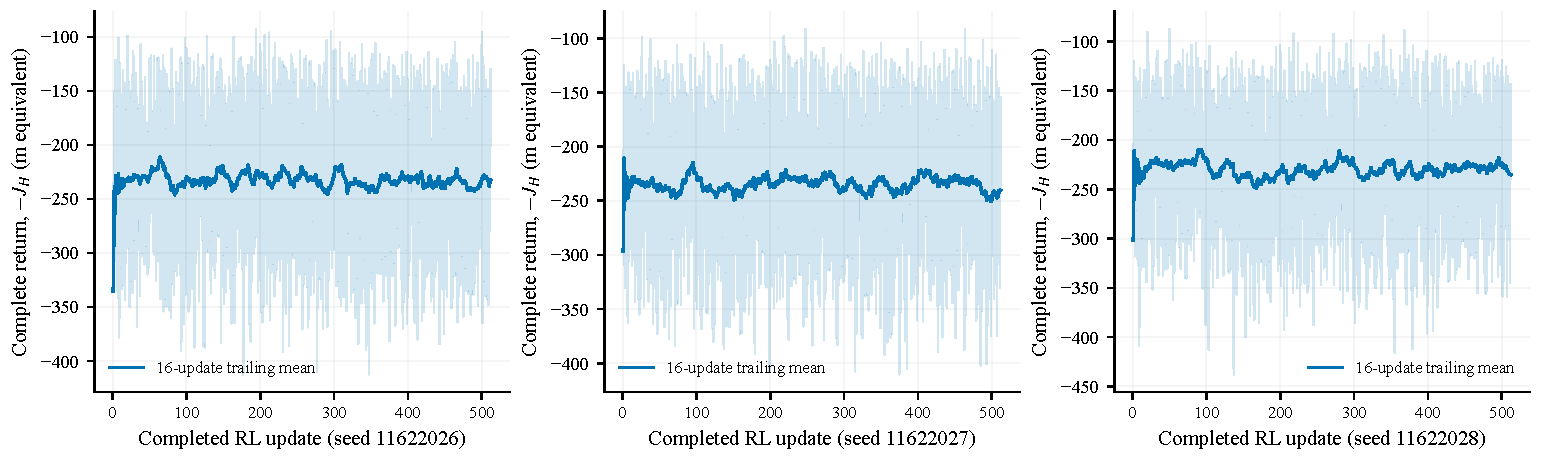
\includegraphics[width=.99\textwidth]{rc3_s2_results_20261107/analysis/figures/fig01_rl_return.pdf}
\caption{Observed complete RL returns across three fixed seeds. Thin traces are arithmetic means over the twelve sampled trajectories per completed update; solid traces use a trailing mean of up to sixteen updates. Inputs change across updates, so these are descriptive training diagnostics rather than paired improvement tests.}
\label{fig:s2-return}
\end{figure*}

\begin{figure*}[t]
\centering
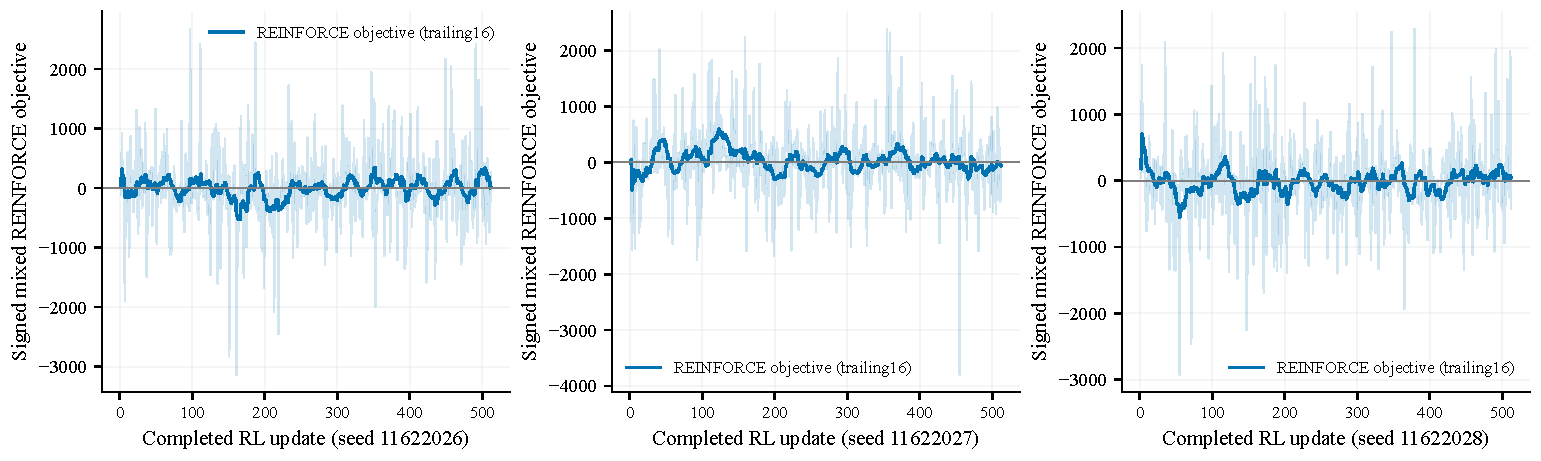
\includegraphics[width=.99\textwidth]{rc3_s2_results_20261107/analysis/figures/fig02_rl_objective.pdf}
\caption{Recorded signed mixed REINFORCE batch objective, with raw and trailing-sixteen-update traces. Its sign and scale depend on detached leave-one-out advantages and sampled log probabilities. This is not a planning-quality metric or comparable to supervised cross-entropy.}
\label{fig:s2-objective}
\end{figure*}

\begin{figure*}[t]
\centering
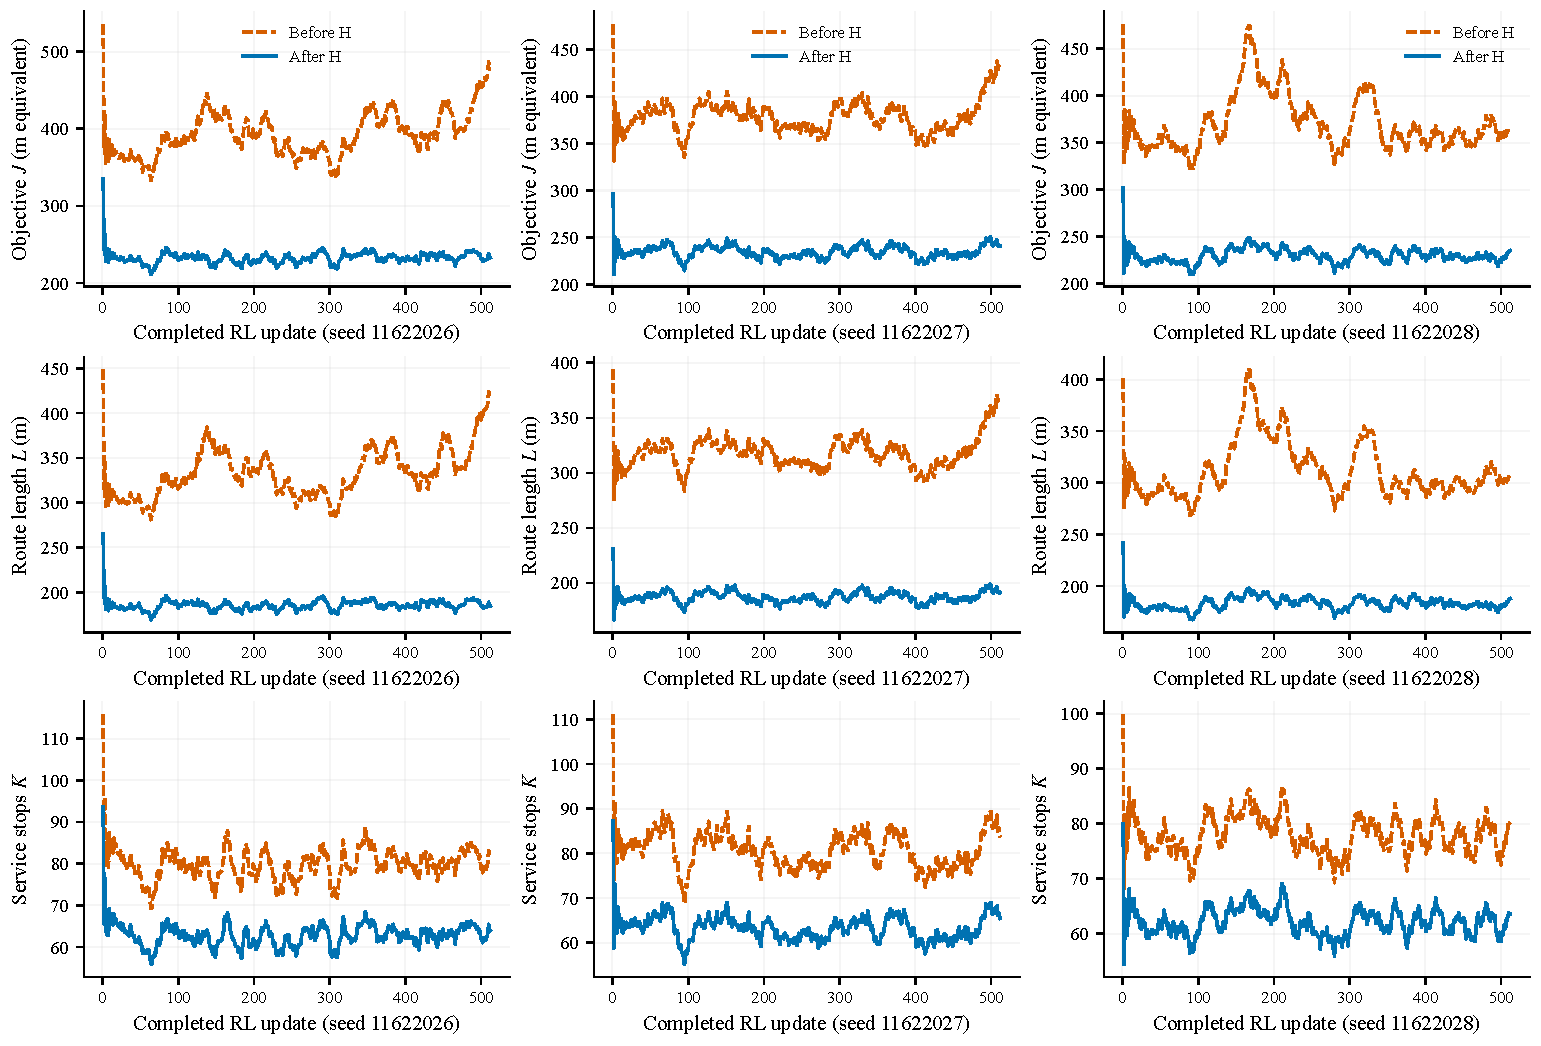
\includegraphics[width=.99\textwidth]{rc3_s2_results_20261107/analysis/figures/fig03_raw_and_H_costs.pdf}
\caption{Observed objective $J=L+0.75K$, route length $L$, and stop count $K$ before and after frozen H, shown as trailing-sixteen-update means. Within-route raw-to-H differences belong to postprocessing; across-update inputs change. Columns show fixed seeds11622026,11622027,11622028.}
\label{fig:s2-costs}
\end{figure*}

\begin{figure*}[t]
\centering
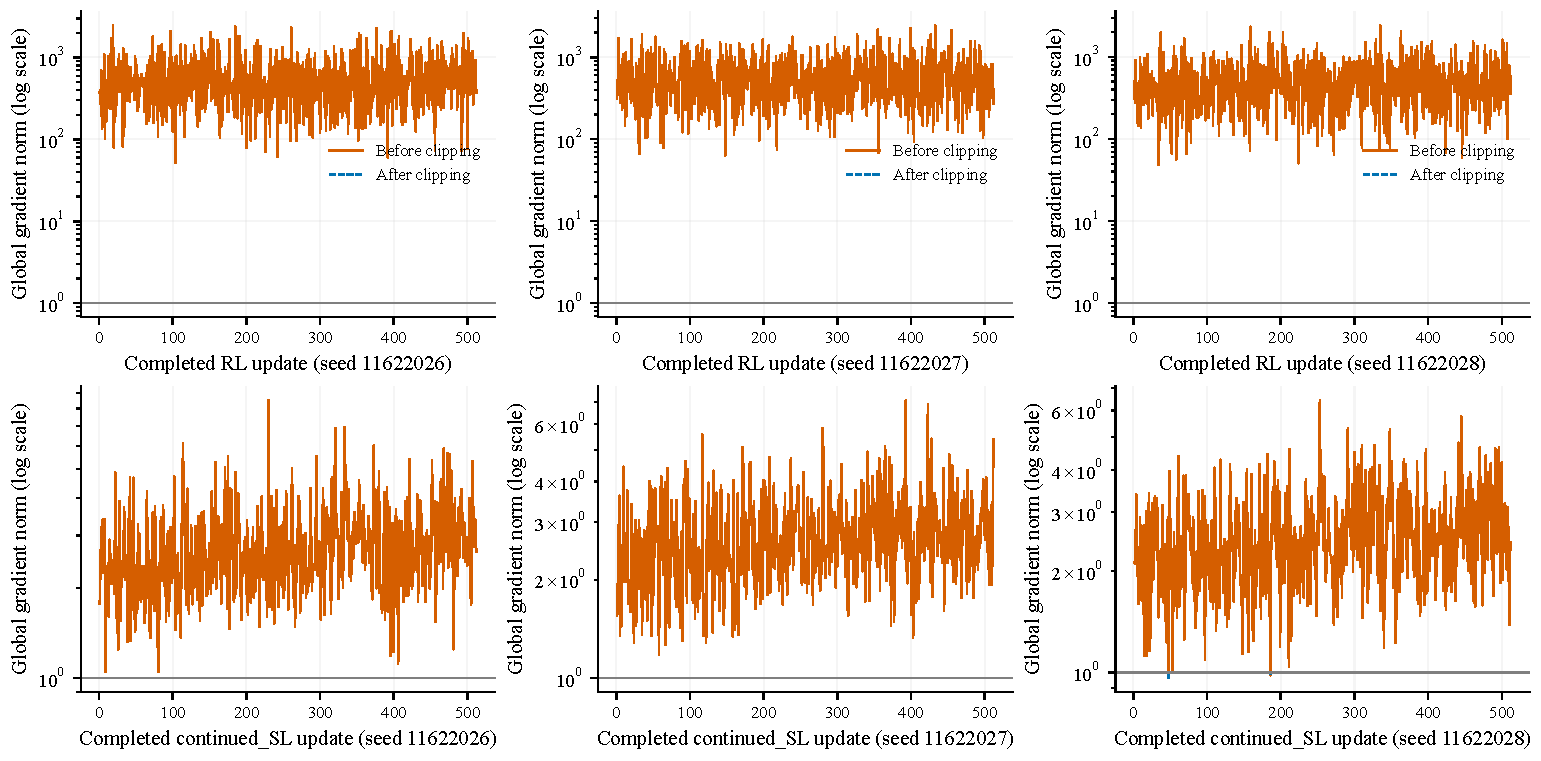
\includegraphics[width=.99\textwidth]{rc3_s2_results_20261107/analysis/figures/fig04_gradient_clipping.pdf}
\caption{Global gradient norms before and after clipping, separately for RL and continued supervised learning. The reference is the approved norm cap1. Exact zero, if present, is plotted at $10^{-14}$ only for log-axis display. These traces verify update mechanics, not planning-quality improvement.}
\label{fig:s2-clipping}
\end{figure*}

\begin{figure*}[t]
\centering
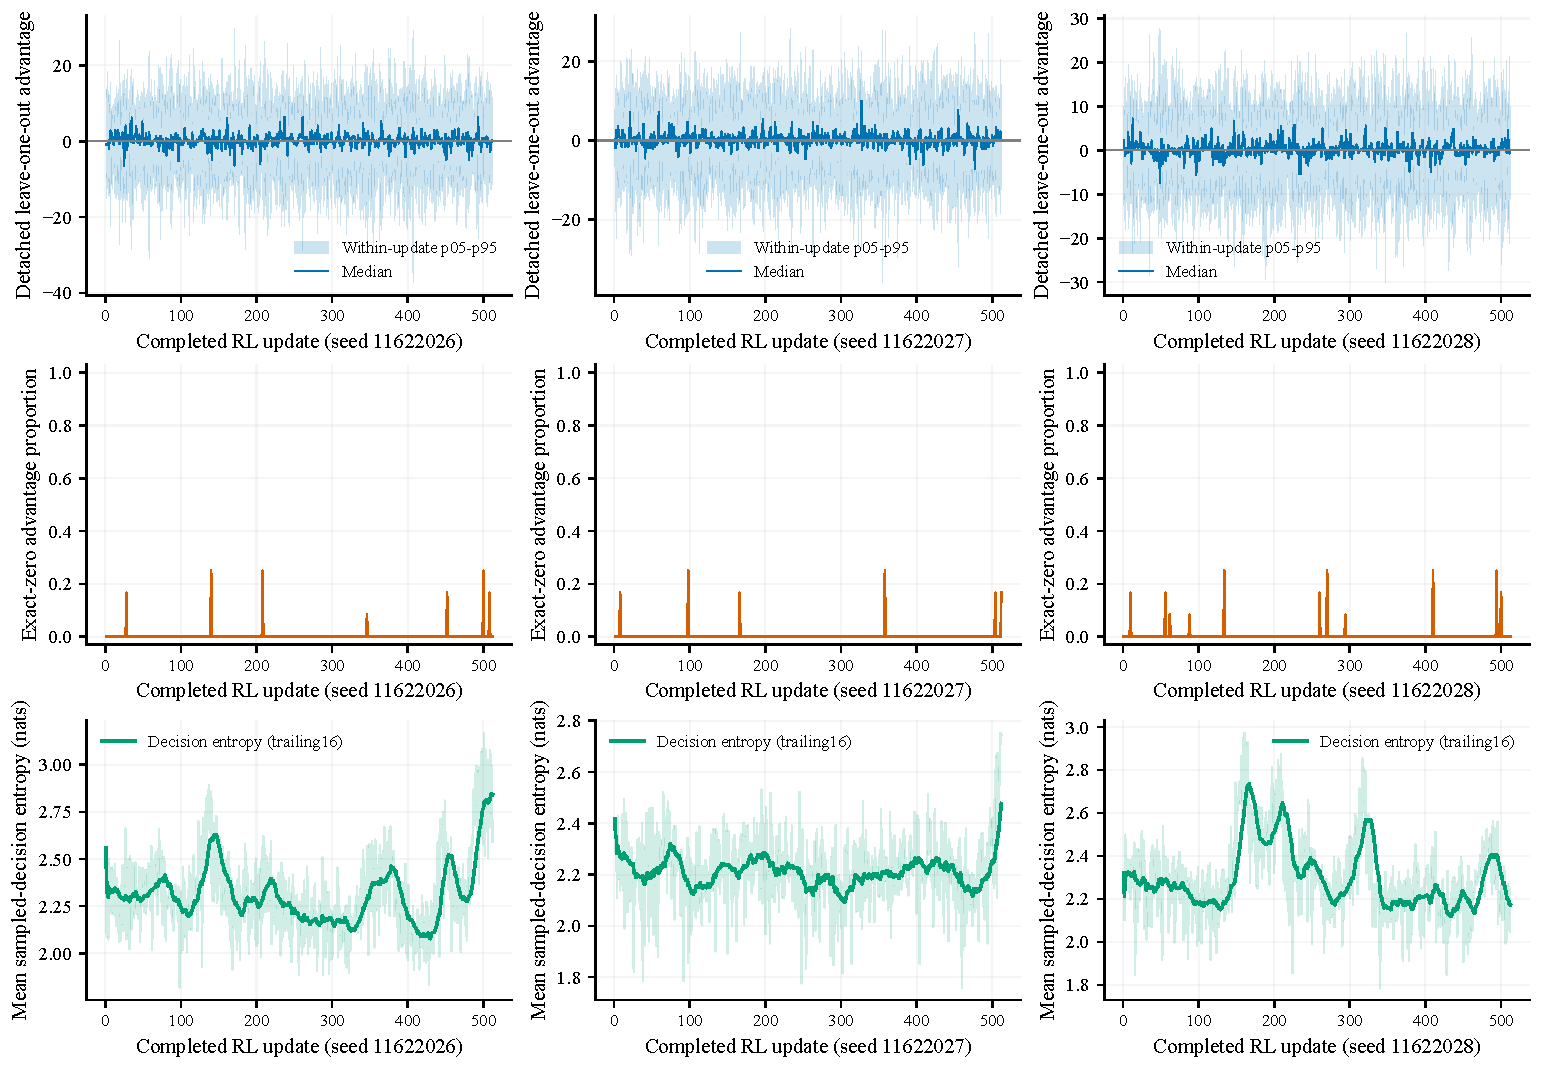
\includegraphics[width=.99\textwidth]{rc3_s2_results_20261107/analysis/figures/fig05_advantage_and_entropy.pdf}
\caption{Within-update detached LOO advantage median and p05--p95 range, exact-zero proportion, and sampled-decision entropy. The range describes twelve dependent sampled trajectories and is not a confidence interval. Forced first actions have no scored entropy.}
\label{fig:s2-signal}
\end{figure*}

\begin{figure*}[t]
\centering
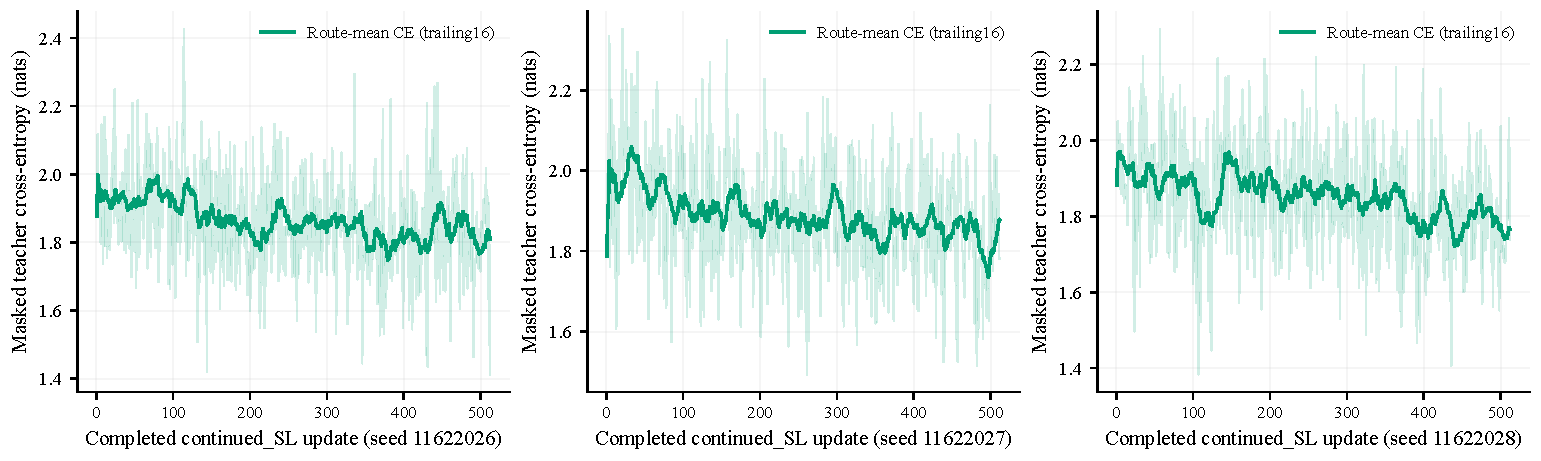
\includegraphics[width=.99\textwidth]{rc3_s2_results_20261107/analysis/figures/fig06_continued_SL_CE.pdf}
\caption{Continued supervised route-mean masked teacher cross-entropy on the fixed saved teacher pool, with raw and trailing-sixteen-update traces. It has a different definition and scale from REINFORCE and does not compare planning performance.}
\label{fig:s2-continued-sl}
\end{figure*}

\begin{figure*}[t]
\centering
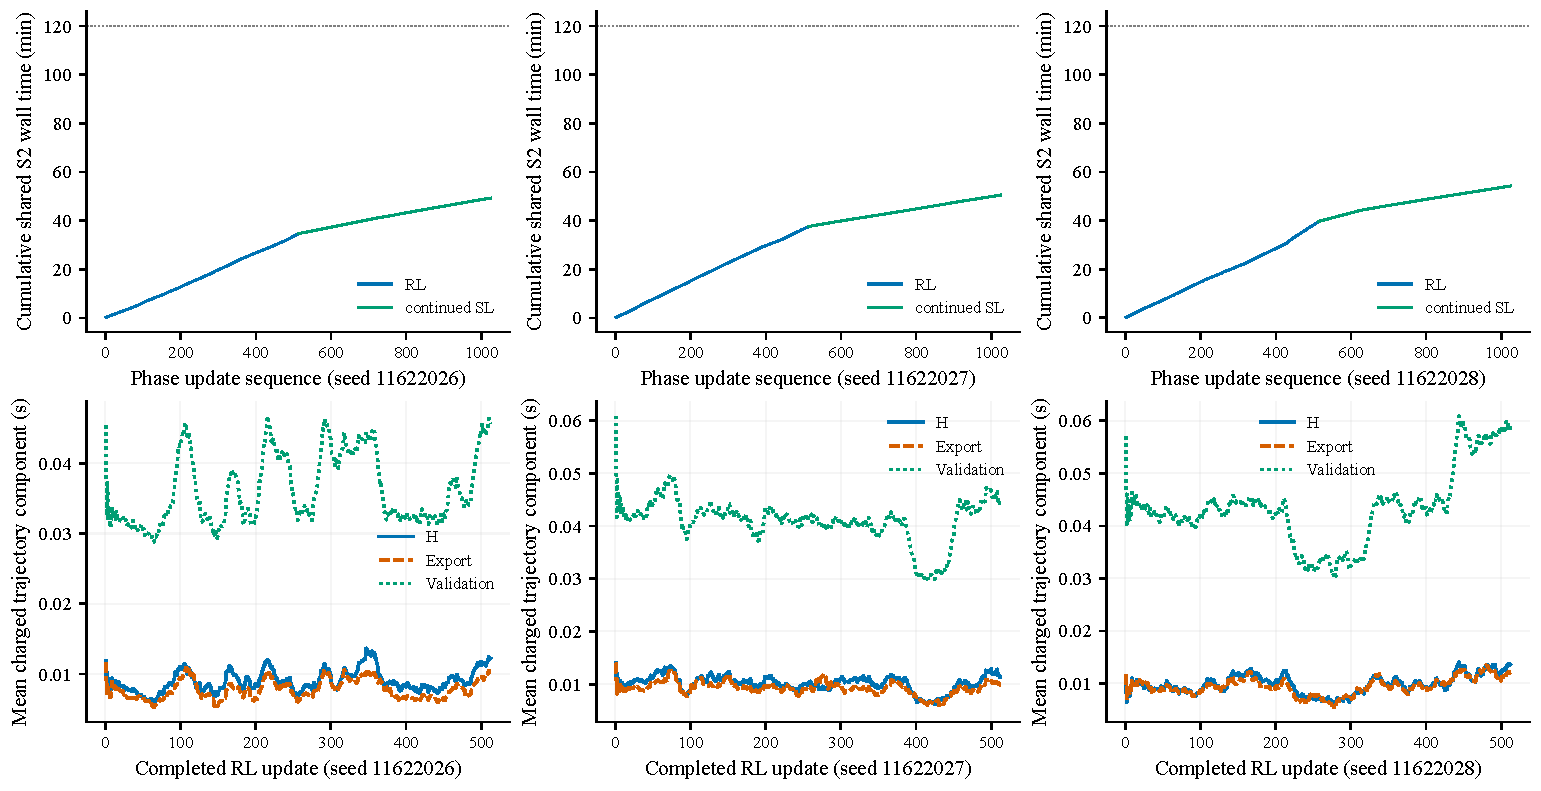
\includegraphics[width=.99\textwidth]{rc3_s2_results_20261107/analysis/figures/fig07_wall_and_terminal_components.pdf}
\caption{Recorded cumulative shared S2 wall time and incremental RL terminal-component time. RL and continued-SL occupy one cumulative clock and must not be added; the reference cap is120min. Lower traces show H/export/validation time per trajectory, including zero incremental time for cache hits. The cumulative ledger separately retains failed, pending, development and final I/O work.}
\label{fig:s2-resources}
\end{figure*}

\begin{figure*}[t]
\centering
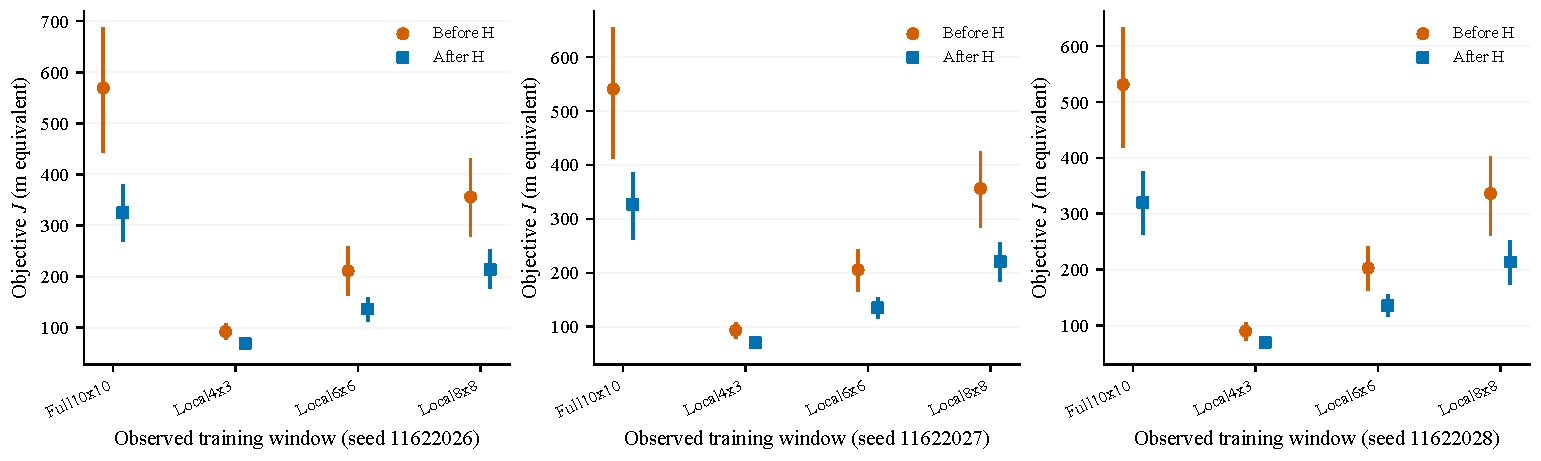
\includegraphics[width=.99\textwidth]{rc3_s2_results_20261107/analysis/figures/fig08_observed_cost_by_window.pdf}
\caption{Observed training objective distributions by task-window size. Points show trajectory means and segments show p25--p75 ranges, before and after frozen H. Ranges are descriptive rather than confidence intervals, and starts from the same instance are dependent. Obstacle-mode and endpoint-condition groups are exported separately. No held-out policy comparison is made.}
\label{fig:s2-window-distribution}
\end{figure*}

\begin{figure*}[t]
\centering
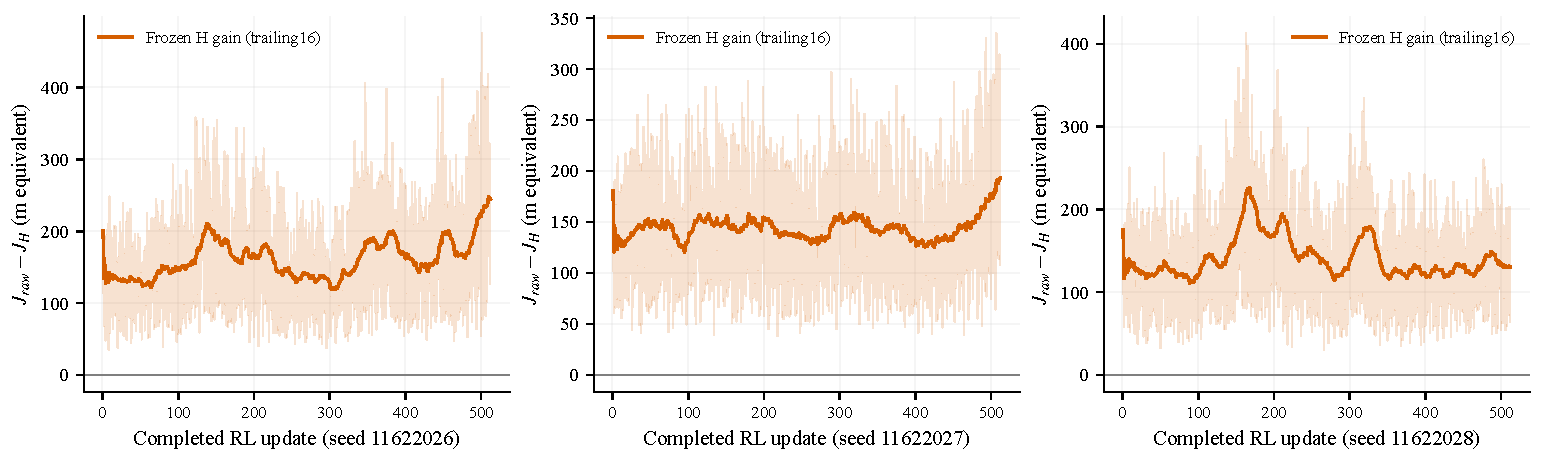
\includegraphics[width=.99\textwidth]{rc3_s2_results_20261107/analysis/figures/fig09_frozen_H_gain.pdf}
\caption{Frozen H's observed contribution, $J_{raw}-J_H$, paired within each recorded trajectory. Thin traces show update means and solid traces show trailing-sixteen-update means. This measures the fixed postprocessor on changing proposals and inputs, not independent network-learning gain.}
\label{fig:s2-h-contribution}
\end{figure*}
